\documentclass[aspectratio=169,11pt]{beamer}
% ==========================================================================
%  KSA lecture-slide theme  =  stock beamer "Boadilla"  +  KSA colour theme
%  brand colours sampled from the official KSA symbol mark:
%    Deep Prussian Blue  #2E3192   (지성 - intellect)
%    Golden Gray         #D6CBB1   (감성 - sensibility)
%  Engine: XeLaTeX.  Usage:
%    \documentclass[aspectratio=169,11pt]{beamer}
%    \input{../../theme/ksa-theme.tex}
%  Each deck lives in its own slides/kor/<deck>/ folder together with its
%  own images; ../../figs/ is kept only as a fallback for the shared cache.
% ==========================================================================

\usepackage{fontspec}
\usepackage{amsmath,amssymb}
\usepackage{graphicx}
\graphicspath{{figs/}{./}{../../../figs/}}
\usepackage{booktabs}
\usepackage{listings}
\usepackage{varwidth}

% ---- fonts (no ctex/xeCJK on this box -> fontspec drives CJK directly) -----
\defaultfontfeatures{Ligatures=TeX}
\setmainfont{Noto Sans CJK KR}
\setsansfont{Noto Sans CJK KR}
\setmonofont{Noto Sans Mono CJK KR}[Scale=0.92]

% ---- base theme: stock Boadilla ------------------------------------------
\usetheme{Boadilla}
\usefonttheme{professionalfonts}
\setbeamertemplate{navigation symbols}{}

% ---- KSA colour theme (recolour the stock theme) --------------------------
\definecolor{ksablue}{HTML}{2E3192}
\definecolor{ksabluedk}{HTML}{20226A}
\definecolor{ksagold}{HTML}{D6CBB1}
\definecolor{ksagolddk}{HTML}{A9976B}
\definecolor{ksared}{HTML}{C0392B}
\definecolor{ksagray}{HTML}{5B5B5B}

\setbeamercolor{structure}{fg=ksablue}
\setbeamercolor{alerted text}{fg=ksared}

\setbeamercolor{palette primary}{fg=white,           bg=ksablue}
\setbeamercolor{palette secondary}{fg=white,         bg=ksablue!85!black}
\setbeamercolor{palette tertiary}{fg=white,          bg=ksabluedk}
\setbeamercolor{titlelike}{fg=ksablue}
\setbeamercolor{frametitle}{fg=ksablue,bg=}
\setbeamercolor{title}{fg=ksablue}
\setbeamercolor{author}{fg=ksagray}
\setbeamercolor{institute}{fg=ksagray}
\setbeamercolor{block title}{fg=white,bg=ksablue}
\setbeamercolor{block body}{fg=black!85,bg=ksablue!6}
\setbeamercolor{item}{fg=ksablue}
\setbeamercolor{section in toc}{fg=black!85}

\setbeamerfont{frametitle}{series=\bfseries}
\setbeamerfont{title}{series=\bfseries}

% ---- footline:  KSA mark | "Made by ..." | n / N   (matches reference) ----
\newcommand{\ksacredit}{}
\setbeamertemplate{footline}{%
  \hbox{%
    \begin{beamercolorbox}[wd=.18\paperwidth,ht=2.6ex,dp=1.5ex,leftskip=1.1em]{}%
      \raisebox{-0.35ex}{\includegraphics[height=2.0ex]{ksa-logo.png}}%
    \end{beamercolorbox}%
    \begin{beamercolorbox}[wd=.64\paperwidth,ht=2.6ex,dp=1.5ex,center]{}%
      {\scriptsize\color{ksagray}\ksacredit}%
    \end{beamercolorbox}%
    \begin{beamercolorbox}[wd=.18\paperwidth,ht=2.6ex,dp=1.5ex,rightskip=1.1em]{}%
      \hfill{\scriptsize\color{ksablue}\insertframenumber\,/\,\inserttotalframenumber}%
    \end{beamercolorbox}%
  }%
  \vskip2pt
}

% ---- section divider: stock \sectionpage, KSA-coloured -------------------
\setbeamertemplate{section page}{%
  \begingroup\centering
    {\color{ksagolddk}\rule{0.16\paperwidth}{1pt}}\par\vskip1.0em
    {\usebeamerfont{title}\color{ksablue}\insertsectionhead\par}\vskip1.0em
    {\color{ksagolddk}\rule{0.16\paperwidth}{1pt}}\par
  \endgroup
}
\AtBeginSection[]{\begin{frame}[plain,noframenumbering]\vfill\sectionpage\vfill\end{frame}}

% ---- code listings ------------------------------------------------------------
\lstdefinestyle{ksa}{%
  basicstyle=\ttfamily\scriptsize,
  keywordstyle=\color{ksablue}\bfseries,
  commentstyle=\color{ksagray}\itshape,
  stringstyle=\color{ksagolddk},
  numberstyle=\tiny\color{ksagray},
  backgroundcolor=\color{ksablue!6},
  frame=leftline, framerule=1.4pt, rulecolor=\color{ksablue},
  xleftmargin=1em, aboveskip=0.8em, belowskip=0.4em,
  showstringspaces=false, breaklines=true, language=Python,
}
\lstset{style=ksa}

% ---- handy macros -----------------------------------------------------------
\newcommand{\kb}[1]{\textbf{\color{ksablue}#1}}   % blue keyword
\newcommand{\kq}[1]{\textbf{\color{ksared}#1}}    % red key-question

\setbeamerfont{title}{series=\bfseries,size=\fontsize{24}{30}\selectfont}
\setbeamerfont{subtitle}{series=\bfseries,size=\fontsize{14}{18}\selectfont}
\setbeamerfont{author}{size=\normalsize}
\setbeamerfont{institute}{size=\small}
\graphicspath{{figs/}{../../../../assets/}}
\makeatletter
\newcommand{\markpage}[1]{\protected@write\@auxout{}{\string\newlabel{#1}{{\the\c@framenumber}{}}}\hypertarget{#1}{}}
\newcommand{\pref}[1]{\hyperlink{#1}{\textcolor{ksagolddk}{(p.\ref{#1})}}}
\makeatother

\renewcommand{\ksacredit}{Machine Learning 1 \,\textperiodcentered\, GBDT와 SHAP}
\title{GBDT 와 SHAP}
\subtitle{앞 나무의 실수를 고쳐 가는 숲, 그리고 ``왜 그렇게 답했나''}
\author{Machine Learning 1}
\institute{한국과학영재학교 (KSA)}
\date{}
\begin{document}
\begin{frame}[plain,noframenumbering]\titlepage\end{frame}

% --- 오늘의 질문
\begin{frame}{오늘의 질문}
\vfill
\centering
{\Large 타이타닉 승객 두 명. 둘 다 \textbf{26살}.}\\[1.0em]
{\LARGE AI 가 본 생존 확률: \quad \kb{96\%} \quad vs \quad \kq{13\%}}\\[1.0em]
{\large 무엇이 둘을 갈랐을까? \quad AI 의 답을 \textbf{이유별로} 나눌 수 있을까?}
\vfill
\note{타이타닉 승객 두 명이 있습니다. 둘 다 26살입니다. 승객 1309명으로 학습한 AI가 본 생존 확률은 한 명은 96퍼센트, 다른 한 명은 13퍼센트입니다. 무엇이 둘을 갈랐을까요? 오늘은 두 가지를 배웁니다. 하나는 이 AI, 표 데이터에서 가장 강력한 모델 중 하나인 GBDT입니다. 다른 하나는 AI의 답을 이유별 점수로 나눠 왜 그렇게 답했는지 보여 주는 도구, SHAP입니다.}
\end{frame}

% --- 부스팅 아이디어
\begin{frame}{부스팅: 앞 나무가 틀린 만큼을 다음 나무가 고친다}
\markpage{boost}
\vfill
\centering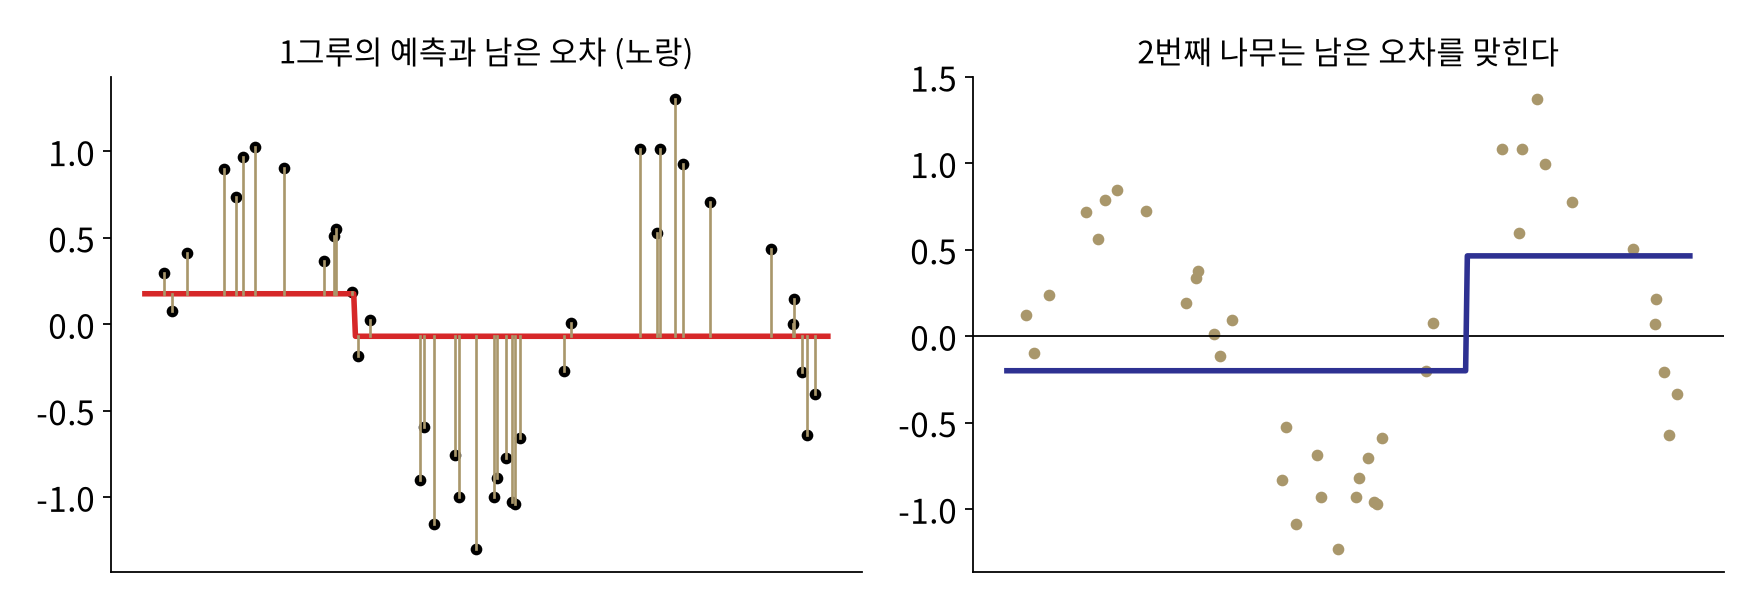
\includegraphics[width=0.84\linewidth]{gb_residual.png}\par\vskip0.2em
{\large 랜덤 포레스트: \textbf{동시에} 키워 투표 \qquad 부스팅: \kb{차례로} 키워 \textbf{더한다}}
\vfill
\note{지난 시간 랜덤 포레스트는 나무를 동시에, 서로 독립적으로 키워 투표했습니다. 부스팅은 나무를 차례로 키웁니다. 먼저 아주 작은 나무 하나로 예측합니다. 왼쪽 그림의 빨간 선입니다. 노란 선이 아직 남은 오차입니다. 두 번째 나무는 원래 답이 아니라 이 남은 오차를 맞히도록 학습합니다. 오른쪽 파란 선입니다. 그리고 첫 나무의 예측에 두 번째 나무의 예측을 더합니다. 그러면 남은 오차가 줄어들고, 세 번째 나무는 또 그 남은 오차를 맞힙니다. 이렇게 앞 나무가 틀린 만큼을 다음 나무가 고쳐 나갑니다.}
\end{frame}

% --- 쌓으면
\begin{frame}{작은 나무를 쌓아 가면}
\vfill
\centering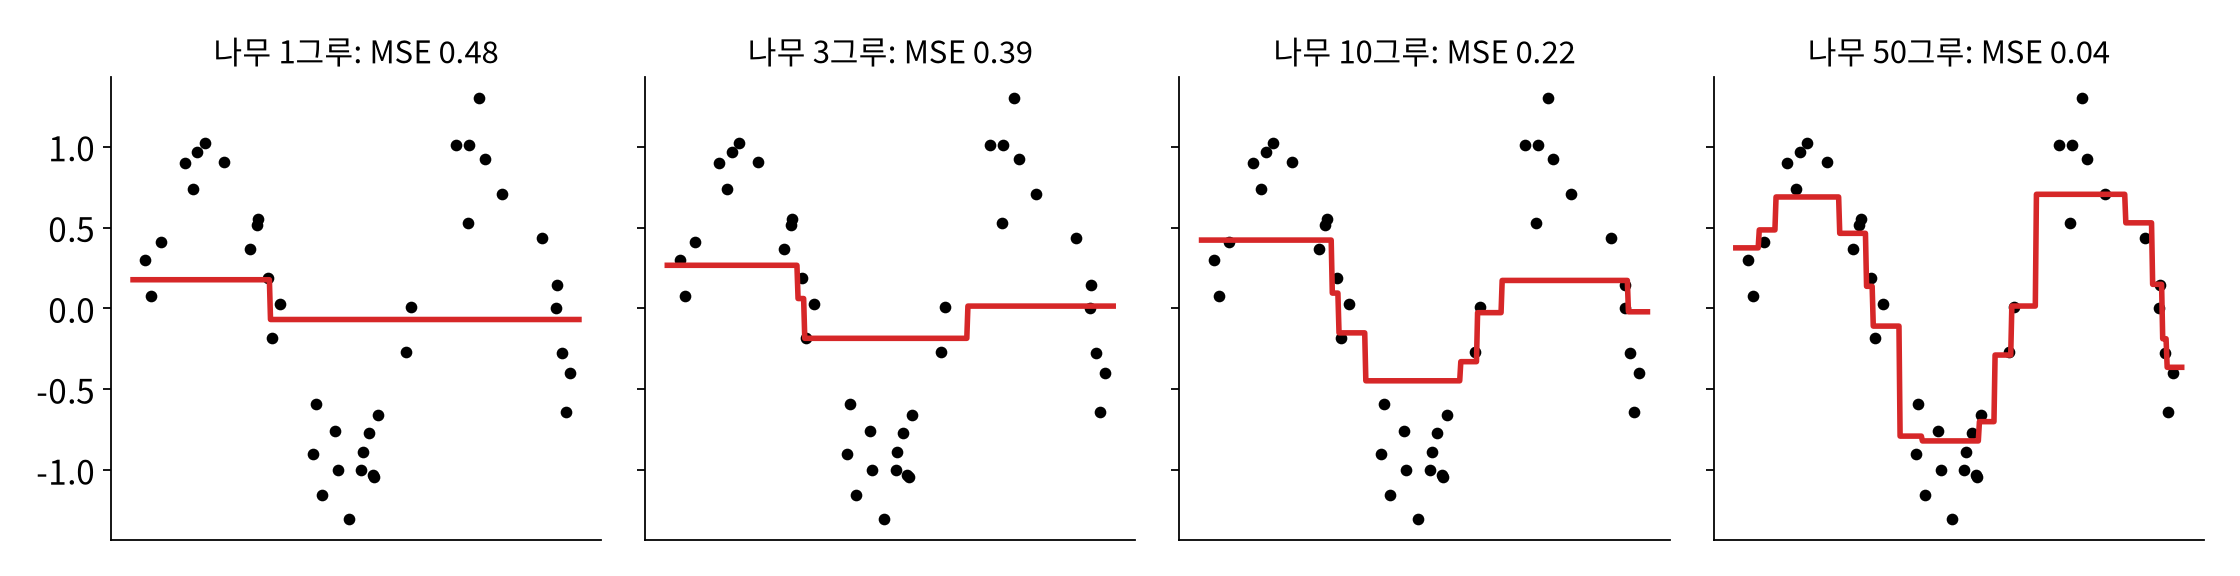
\includegraphics[width=0.96\linewidth]{gb_toy.png}\par\vskip0.2em
{\large 질문 하나짜리 나무도 50그루 쌓으면 \quad 학습 MSE 0.48 $\to$ 0.39 $\to$ 0.22 $\to$ \kb{0.04}}
\vfill
\note{질문 하나짜리, 깊이 1인 아주 작은 나무로 물결 모양 데이터를 맞춰 봤습니다. 한 그루는 계단 하나뿐이라 학습 오차가 0.48입니다. 3그루, 10그루, 50그루로 쌓을수록 계단이 늘면서 물결을 따라가고, 오차가 0.04까지 줄어듭니다. 하나하나는 약한 나무지만 쌓으면 강해집니다. 그래서 부스팅, 끌어올리기라는 이름이 붙었습니다.}
\end{frame}

% --- 식
\begin{frame}{식으로: 그레이디언트 부스팅}
\vfill
\centering
{\LARGE\[ F_m(x) = F_{m-1}(x) + \textcolor{ksared}{\eta}\, h_m(x) \]}\vskip0.4em
\renewcommand{\arraystretch}{1.3}
{\large\begin{tabular}{ll}
$F_{m-1}$ & 지금까지 쌓은 나무들의 예측 합\\
$h_m$ & 새 나무: 지금의 \textbf{남은 오차} (손실의 기울기 반대 방향) 를 맞히도록 학습\\
\textcolor{ksared}{$\eta$} & 학습률: 새 나무를 얼마나 믿을지 (보통 0.01 $\sim$ 0.3)
\end{tabular}}\vskip0.6em
{\large GBDT = Gradient Boosting Decision Tree \quad 경사하강법을 \textbf{함수} 공간에서 하는 것}
\vfill
\note{식으로 쓰면 이렇습니다. 지금까지 쌓은 나무들의 예측 F에, 새 나무 h의 예측에 학습률 에타를 곱해 더합니다. 새 나무는 지금 남은 오차를 맞히도록 학습합니다. 제곱 오차일 때 남은 오차는 손실을 예측값으로 미분한 기울기의 반대 방향과 같습니다. 그래서 경사하강법처럼 기울기 반대로 조금씩 움직이는데, 가중치가 아니라 예측 함수 자체를 움직인다고 보면 됩니다. 이름이 그레이디언트 부스팅 결정 트리, GBDT인 이유입니다. 학습률은 새 나무를 얼마나 믿을지로, 작게 할수록 나무가 많이 필요하지만 더 안정적입니다.}
\end{frame}

% --- 타이타닉 GBDT
\begin{frame}{타이타닉 GBDT}
\vfill
\centering
\renewcommand{\arraystretch}{1.4}
{\large\begin{tabular}{ll}
데이터 & 승객 1,309명, 특징 5개: 등급 · 성별 · 나이 · 요금 · 가족 수\\
모델 & 깊이 3 나무 \textbf{200그루}, 학습률 0.05\\
학습 데이터 오답률 & 1그루 38.2\% $\to$ 10그루 20.1\% $\to$ 200그루 \kb{13.9\%}\\
5겹 교차 검증 정확도 & \kb{80.7\%}
\end{tabular}}\vskip0.8em
{\large 그런데 200그루의 합이라 \kq{왜 그렇게 답했는지 보이지 않는다}}
\vfill
\note{타이타닉 승객 1309명의 등급, 성별, 나이, 요금, 가족 수로 생존을 예측하는 GBDT를 만들었습니다. 깊이 3짜리 나무 200그루를 학습률 0.05로 쌓았습니다. 학습 데이터 오답률은 1그루일 때 38퍼센트에서 10그루에 20퍼센트, 200그루에 14퍼센트로 줄었습니다. 처음 보는 승객에 대한 교차 검증 정확도는 80.7퍼센트입니다. 문제는 이 답이 나무 200그루의 합이라서, 결정 트리 한 그루처럼 왜 그렇게 답했는지 읽을 수 없다는 겁니다. 그래서 SHAP이 필요합니다.}
\end{frame}

% --- RF vs GBDT
\begin{frame}{랜덤 포레스트 vs GBDT}
\vfill
\centering
\renewcommand{\arraystretch}{1.5}
{\large\begin{tabular}{lll}
 & 랜덤 포레스트 & GBDT\\\hline
나무 키우기 & 동시에, 독립적으로 & \kb{차례로}, 앞 나무의 실수를 보고\\
나무 크기 & 깊게 (끝까지) & 얕게 (깊이 3 $\sim$ 8)\\
줄이는 것 & 분산 (흔들림) & 편향 (덜 배움)\\
나무를 늘리면 & 안정될 뿐 & \kq{과대적합될 수 있다} $\to$ 조기 종료\\
튜닝 & 거의 필요 없음 & 학습률 · 나무 수 · 깊이
\end{tabular}}\vskip0.6em
{\small XGBoost, LightGBM, CatBoost: GBDT 를 빠르게 만든 라이브러리, 표 데이터 대회의 단골}
\vfill
\note{지난 시간의 랜덤 포레스트와 비교해 봅니다. 랜덤 포레스트는 깊은 나무를 동시에 키워 평균을 내서 흔들림, 즉 분산을 줄입니다. GBDT는 얕은 나무를 차례로 키워 덜 배운 부분, 즉 편향을 줄입니다. 그래서 랜덤 포레스트는 나무를 늘려도 안정될 뿐이지만, GBDT는 나무를 너무 많이 쌓으면 학습 데이터의 잡음까지 맞혀서 과대적합될 수 있습니다. 6주차에 배운 조기 종료를 여기서 씁니다. 튜닝할 것도 학습률, 나무 수, 깊이로 더 많습니다. 대신 잘 튜닝하면 표 데이터에서 가장 강력한 모델 중 하나이고, XGBoost나 LightGBM 같은 라이브러리가 데이터 대회의 단골입니다.}
\end{frame}

% --- SHAP 아이디어
\begin{frame}{SHAP: 정보를 하나씩 알려 주며 확률이 오른 만큼을 잰다}
\markpage{idea}
\vfill
\centering
{\large 1등석 여성 승객 (26살). 정보를 하나씩 알려 준다:}\vskip0.5em
\renewcommand{\arraystretch}{1.35}
{\large\begin{tabular}{lcc}
아는 정보 & 생존 확률 & 오른 만큼\\\hline
아무것도 모름 (승객 평균) & 38.2\% & \\
+ 성별 (여성) & 68.8\% & \kb{+30.6}\\
+ 등급 (1등석) & 87.8\% & \kb{+19.0}\\
+ 나머지 (나이 · 요금 · 가족) & 96.0\% & +8.2
\end{tabular}}\vskip0.5em
{\large 그런데 \textbf{순서}를 바꾸면 오른 만큼이 달라진다 \quad (등급부터 알려 주면 등급 +13.1)}
\vfill
\note{SHAP의 아이디어는 간단합니다. 승객 정보를 하나씩 알려 주며 생존 확률이 오른 만큼을 그 정보의 몫으로 봅니다. 1등석 여성 승객에 대해 아무것도 모르면 승객 평균 38.2퍼센트입니다. 여성이라는 걸 알려 주면 68.8퍼센트로 30.6만큼 오릅니다. 1등석이라는 것까지 알려 주면 87.8퍼센트로 19.0, 나머지까지 알려 주면 96퍼센트로 8.2 오릅니다. 그런데 문제가 있습니다. 순서를 바꿔 등급부터 알려 주면 38.2에서 51.3으로 등급의 몫이 13.1이 됩니다. 순서에 따라 몫이 달라집니다.}
\end{frame}

% --- 섀플리 값
\begin{frame}{해결: 모든 순서의 평균 (섀플리 값)}
\markpage{shapley}
\vfill
\centering
{\LARGE\[ \phi_j = \frac{1}{\text{순서의 수}}\sum_{\text{모든 순서}} \big(\text{$j$ 를 알려 줬을 때 오른 만큼}\big) \]}\vskip0.4em
{\large 정보 3가지 $\to$ 순서 $3! = 6$ 가지 \quad 1등석 여성: \kb{성별 $+34.0$, 등급 $+22.6$, 나머지 $+1.3$}}\\[0.6em]
{\large 평균 38.2 $+$ 34.0 $+$ 22.6 $+$ 1.3 $= \kb{96.0}$ \quad 몫의 합 = \textbf{정확히} 모델의 답}\\[0.4em]
{\small 게임 이론의 공정한 기여 나누기 (Shapley, 1953) \quad SHAP = SHapley Additive exPlanations (Lundberg \& Lee, 2017)}
\vfill
\note{해결책은 모든 순서를 다 해 보고 평균을 내는 겁니다. 정보가 성별, 등급, 나머지 셋이면 알려 주는 순서는 3 팩토리얼, 6가지입니다. 6가지 순서에서 각 정보가 확률을 올린 만큼을 평균 내면 성별 34.0, 등급 22.6, 나머지 1.3이 나옵니다. 중요한 성질이 있습니다. 평균 38.2에 세 몫을 더하면 정확히 96.0, 모델의 답이 됩니다. 이 방법은 게임 이론에서 팀원들의 기여를 공정하게 나누려고 섀플리가 1953년에 만든 섀플리 값이고, 그는 이 연구 등으로 2012년 노벨 경제학상을 받았습니다. 이를 머신러닝 설명에 쓴 것이 SHAP입니다.}
\end{frame}

% --- 모르는 정보
\begin{frame}{``모르는 정보''는 어떻게 처리하나}
\vfill
\centering
{\large 모델은 성별을 꼭 넣어야 답한다. 성별을 ``모른다''는 건?}\vskip0.6em
{\Large 성별 자리에 \textbf{여러 승객의 실제 성별}을 넣어 보고 평균}\\[0.8em]
{\large 나무로 보면: 모르는 질문에서는 \textbf{양쪽 길을 다 가서} 비율대로 섞는다}\\[0.4em]
{\large 1등석 여성: 다 알면 93\% \quad 성별을 모르면 남 64 · 여 36 비율로 섞어 \kq{44\%}}\\[0.6em]
{\small (깊이 2 짜리 설명용 나무 하나로 계산한 예)}
\vfill
\note{그런데 성별을 모른다는 건 어떻게 계산할까요? 모델은 성별 칸에 값이 있어야 답할 수 있습니다. SHAP은 성별 자리에 여러 승객의 실제 성별을 넣어 보고 그 답들을 평균 냅니다. 나무 하나로 보면, 모르는 질문에서는 양쪽 길을 다 가서 승객 비율대로 섞는 셈입니다. 설명용으로 깊이 2짜리 나무를 하나 만들어 보면, 1등석 여성은 다 알 때 생존 93퍼센트인 잎으로 갑니다. 성별을 모르면 남자 쪽 길과 여자 쪽 길을 승객 비율 64 대 36으로 섞어서 44퍼센트가 됩니다.}
\end{frame}

% --- 두 승객
\begin{frame}{두 승객의 몫}
\markpage{two}
\vfill
\centering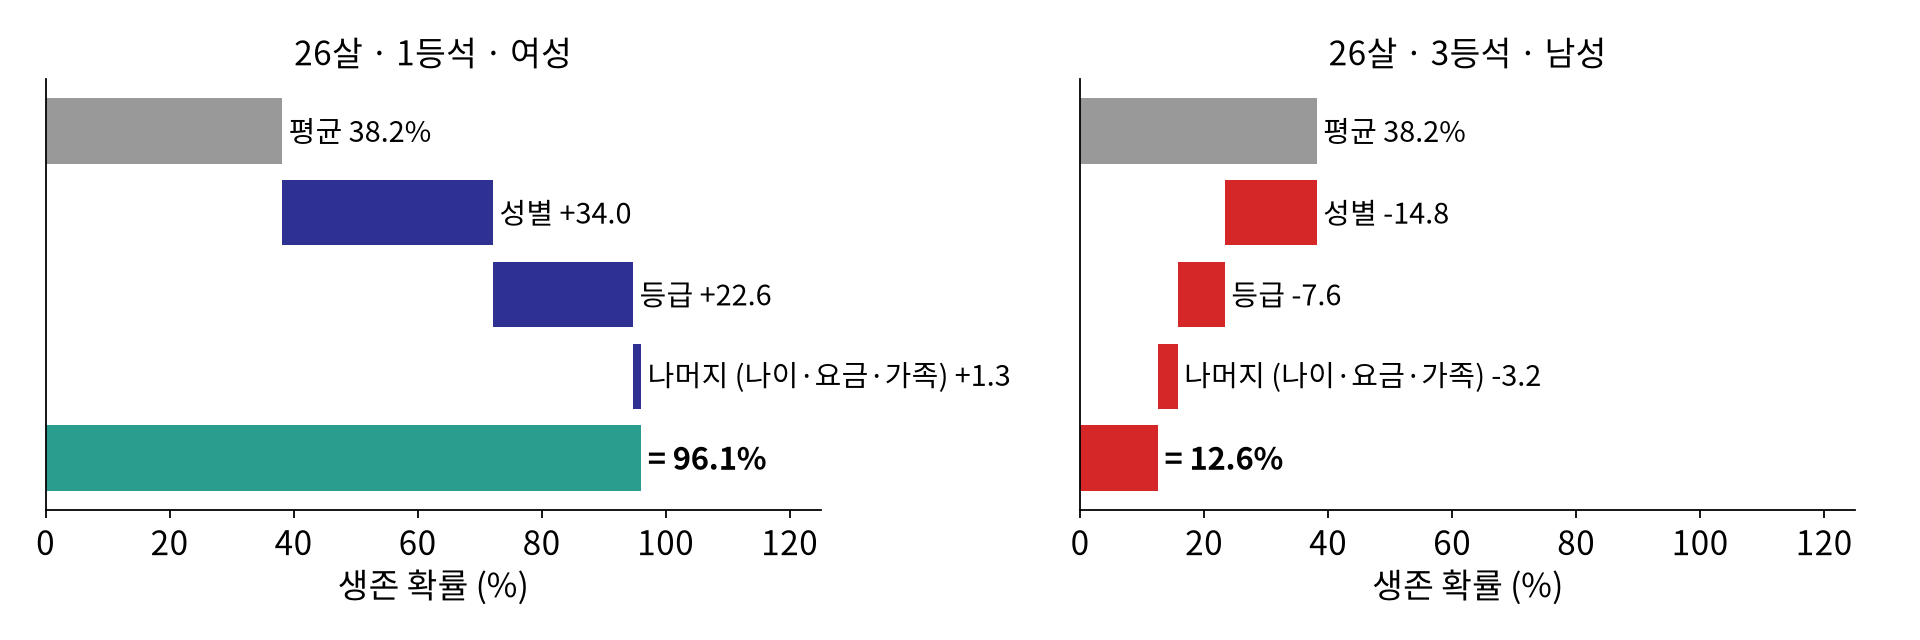
\includegraphics[width=0.94\linewidth]{gb_waterfall.png}\par\vskip0.2em
{\large 같은 26살, \textbf{성별} ($+34.0$ vs $-14.8$) 과 \textbf{등급} ($+22.6$ vs $-7.6$) 이 갈랐다}\\[0.2em]
{\small 그날 밤 여성과 아이를 먼저 구명보트에 태웠다고 알려져 있다}
\vfill
\note{두 승객의 몫을 나란히 놓았습니다. 왼쪽 1등석 여성은 평균 38.2에서 성별로 34, 등급으로 22.6을 얻어 96퍼센트입니다. 오른쪽 3등석 남성은 성별로 14.8, 등급으로 7.6, 나머지로 3.2를 잃어 12.7퍼센트입니다. 같은 26살인데 둘을 가른 가장 큰 이유는 성별, 그다음은 등급입니다. 그날 밤 여성과 아이를 먼저 구명보트에 태웠고, 1등석 객실이 갑판에 가까웠다고 알려져 있습니다. 모델이 데이터에서 그 패턴을 배운 겁니다.}
\end{frame}

% --- 전체
\begin{frame}{모든 승객으로 모아 보면}
\vfill
\centering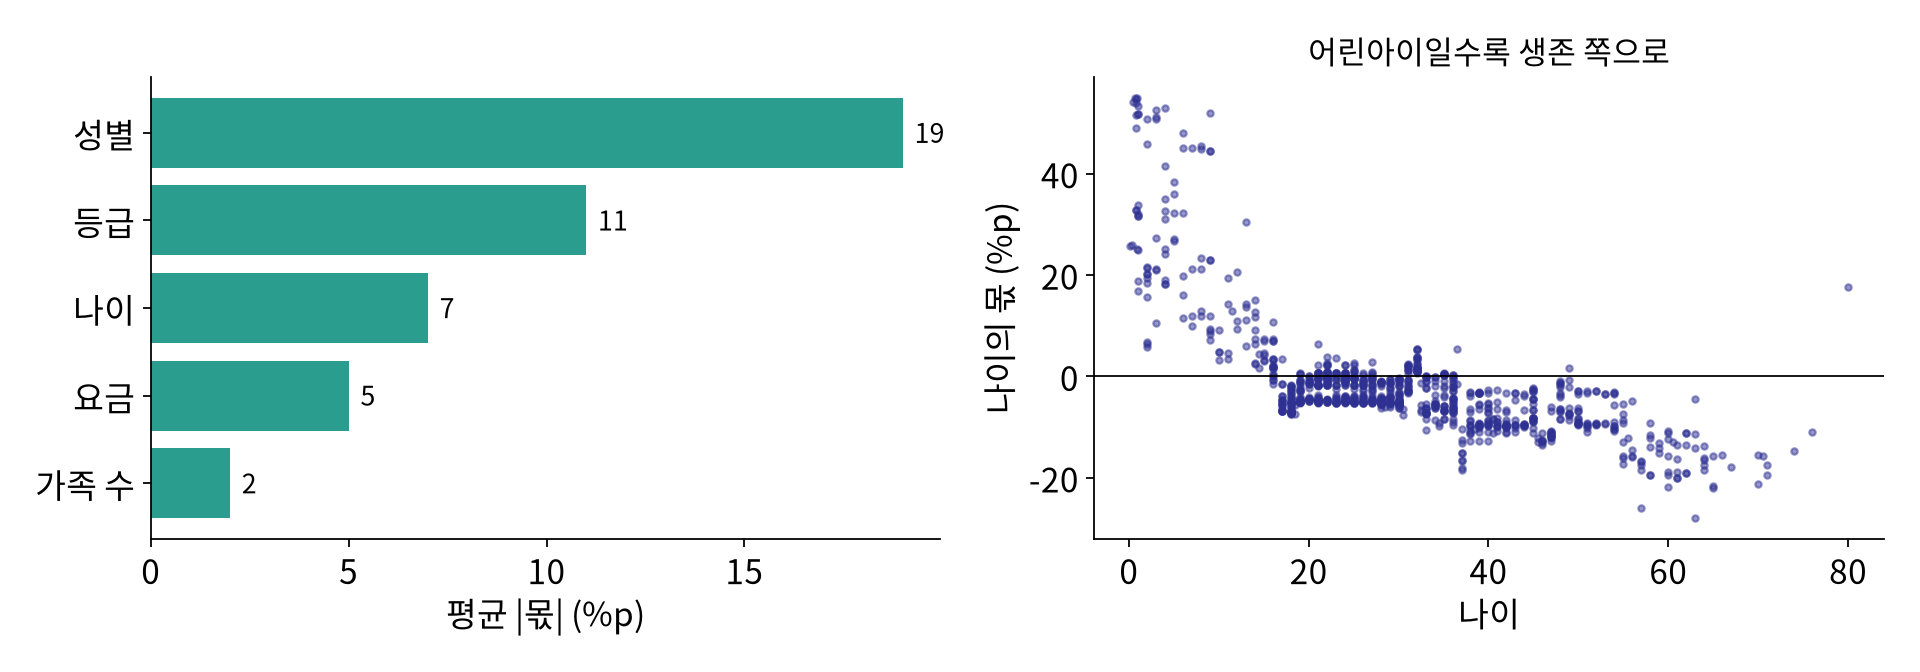
\includegraphics[width=0.84\linewidth]{gb_global.png}\par\vskip0.2em
{\large 평균 $|$몫$|$ (\%p): 성별 \kb{19} \; 등급 11 \; 나이 7 \; 요금 5 \; 가족 2}
\vfill
\note{승객 1309명 모두의 SHAP 값을 모으면 모델 전체를 이해할 수 있습니다. 왼쪽은 각 정보의 몫의 크기를 평균 낸 것입니다. 성별이 평균 19퍼센트포인트로 가장 크고, 등급 11, 나이 7, 요금 5, 가족 수 2입니다. 지난 시간 랜덤 포레스트의 불순도 기반 중요도에서는 요금이 1등이었는데, SHAP은 성별을 1등으로 봅니다. 값의 종류가 많은 요금을 과대평가하는 문제가 SHAP에는 없습니다. 오른쪽은 나이의 몫을 나이별로 찍은 것입니다. 10살 미만 어린아이들은 나이 덕분에 생존 쪽으로 크게 올라갑니다. 아이를 먼저 구했다는 이야기와 맞습니다.}
\end{frame}

% --- 주의
\begin{frame}{SHAP 을 읽을 때 주의할 점}
\vfill
\centering
\renewcommand{\arraystretch}{1.5}
{\large\begin{tabular}{ll}
\textbf{모델 설명이다} & 모델이 무엇을 보고 답했는지일 뿐, 원인을 증명하지 않는다\\
\textbf{얽힌 특징} & 등급과 요금처럼 함께 움직이면 몫이 나뉘어 보인다\\
\textbf{계산량} & 정보 $n$ 개면 순서 $n!$ 개 $\to$ 나무는 빠른 공식 (TreeSHAP)
\end{tabular}}\vskip0.8em
{\large SHAP 은 나무뿐 아니라 신경망 (이미지 · 텍스트) 까지 \textbf{어떤 모델에도} 쓸 수 있다}
\vfill
\note{SHAP을 읽을 때 주의할 점이 있습니다. 첫째, SHAP은 모델이 무엇을 보고 답했는지를 설명할 뿐, 세상의 원인을 증명하지 않습니다. 데이터에 편향이 있으면 모델도, SHAP도 그 편향을 그대로 보여 줍니다. 둘째, 등급과 요금처럼 함께 움직이는 특징은 몫이 서로 나뉘어 보여서 하나하나만 보면 오해할 수 있습니다. 셋째, 정보가 n개면 순서가 n 팩토리얼개라 그대로는 계산이 불가능합니다. 나무 모델에는 빠른 공식 TreeSHAP이 있고, 다른 모델은 근사합니다. 그래서 SHAP은 나무뿐 아니라 이미지나 텍스트를 다루는 신경망까지 어떤 모델에도 쓸 수 있습니다.}
\end{frame}

% --- 문제풀이
\begin{frame}{문제풀이}
\vfill
\begin{enumerate}
\item 첫 나무가 모든 승객에게 0.4 를 예측했다. 실제 답이 1, 0, 1 인 세 승객의 남은 오차는? 학습률 0.5 인 두 번째 나무가 이 오차를 정확히 맞히면 새 예측은?\vskip0.8em
\item 정보 A, B 두 개. 아무것도 모를 때 50, A 만 알 때 70, B 만 알 때 60, 둘 다 알 때 90. A 와 B 의 섀플리 값은? 합은?\vskip0.8em
\item GBDT 의 학습률을 0.5 에서 0.05 로 줄였다. 나무 수는 어떻게 해야 하나?
\end{enumerate}
\vfill
\note{1번 답. 남은 오차는 0.6, 마이너스 0.4, 0.6입니다. 학습률 0.5를 곱해 더하면 0.7, 0.2, 0.7이 됩니다. 2번 답. A를 먼저 알려 주는 순서에서 A는 20, B는 20. B를 먼저 알려 주는 순서에서 B는 10, A는 30. 평균하면 A는 25, B는 15이고, 합 40은 90 빼기 50과 같습니다. 3번 답. 한 그루가 고치는 양이 10분의 1로 줄었으니 나무를 그만큼 더 많이 쌓아야 합니다. 보통 조기 종료로 개수를 정합니다.}
\end{frame}

% --- 실습
\begin{frame}{실습}
\vfill
\centering\begin{tabular}{rl}
\large 1 & 부스팅 직접 구현: 깊이 1 나무로 남은 오차를 차례로 맞히기 $\to$ MSE 0.48 $\to$ 0.04\\[0.5em]
\large 2 & 타이타닉 GBDT: 학습률 · 나무 수 바꿔 보기, 조기 종료\\[0.5em]
\large 3 & SHAP: 두 승객의 몫 직접 계산 (6가지 순서) + \texttt{shap} 라이브러리로 확인
\end{tabular}\vskip1em
Titanic (OpenML; Vanderbilt titanic3) \\[0.4em]\href{https://colab.research.google.com/github/SuminHan/book-ml/blob/main/slides/v2/ml1/week07/gbdt_shap/lab/gbdt_shap.ipynb}{\textcolor{ksagolddk}{▶ Colab에서 실습 노트북 열기}}
\vfill
\note{실습은 세 부분입니다. 첫째, 깊이 1짜리 나무로 남은 오차를 차례로 맞히는 부스팅을 직접 구현해서 오늘의 0.48에서 0.04를 재현합니다. 둘째, 타이타닉 GBDT에서 학습률과 나무 수를 바꿔 보고 조기 종료를 써 봅니다. 셋째, 두 승객의 섀플리 값을 6가지 순서로 직접 계산하고, shap 라이브러리의 결과와 비교합니다.}
\end{frame}

% --- 정리
\begin{frame}{정리}
\vfill
\centering\large\begin{tabular}{l}
\textbf{GBDT} \quad 작은 나무를 차례로, 앞의 \textbf{남은 오차}를 맞히며 더한다 ($F \leftarrow F + \eta h$)\\[0.5em]
타이타닉 200그루 · 교차 검증 80.7\% \quad 나무가 많으면 과대적합 $\to$ 조기 종료\\[0.5em]
\textbf{SHAP} \quad 정보를 알려 줄 때 오른 만큼을 \kb{모든 순서로 평균} (섀플리 값)\\[0.5em]
몫의 합 = 모델의 답 \quad 26살 두 승객을 가른 것: 성별 · 등급
\end{tabular}
\vfill
\note{정리합니다. GBDT는 작은 나무를 차례로 키우며, 앞 나무들이 남긴 오차를 다음 나무가 맞혀 더해 가는 모델입니다. 타이타닉에서 200그루로 교차 검증 80.7퍼센트를 얻었고, 나무를 너무 많이 쌓으면 과대적합되니 조기 종료를 씁니다. SHAP은 정보를 하나씩 알려 줄 때 확률이 오른 만큼을 모든 순서로 평균 낸 섀플리 값으로, 몫을 모두 더하면 정확히 모델의 답이 됩니다. 26살 두 승객을 가른 것은 성별과 등급이었습니다.}
\end{frame}
\end{document}
